\documentclass{beamer}
\mode<presentation>
\setbeamertemplate{navigation symbols}{}
\usepackage{graphics}
\usepackage{amsmath}
\usetheme{Warsaw}
%\usetheme{Frankfurt}
%\usepackage{url}
%\usepackage{cite}
\usepackage{multirow}
\usepackage{hyperref}
\usepackage{tcolorbox}
\beamersetuncovermixins{\opaqueness<1>{25}}{\opaqueness<2->{1}}
\begin{document}
\title{Word Search Puzzle (P9)}  
\author{Venkhat V, Pinkesh Barsopia}
%\titlegraphic{\includegraphics[scale=0.2]{iitblogo.jpg}}
\institute{Department of Electrical Engineering\\ Indian Institute of Technology Bombay \\ GitHub link: https://github.com/pinkeshb/SDES\_wordpuzzle/tree/pdev}
\date{April 29, 2013} 

\setbeamercovered{invisible}
\begin{frame}
\titlepage
\end{frame}
% \begin{frame}[shrink]\frametitle{Outline}
% \tableofcontents
% \end{frame} 



\begin{frame}\frametitle{Word Search Puzzle (P9) - Project Aim }
\begin{itemize}
 \item Interactive game based on Classic Word Search Puzzle
\item Search a set of words embedded in a $N \times N$ matrix of characters

\end{itemize}
\pause
\begin{columns}[c]
\begin{column}{5cm}
\begin{block}{Different features}
\begin{enumerate}
\item User selectable difficulty levels, Dictionary, Grid Size
\item Score
\item Time limit
\end{enumerate}
\end{block}
\end{column}

\begin{column}{5cm}

\begin{figure}
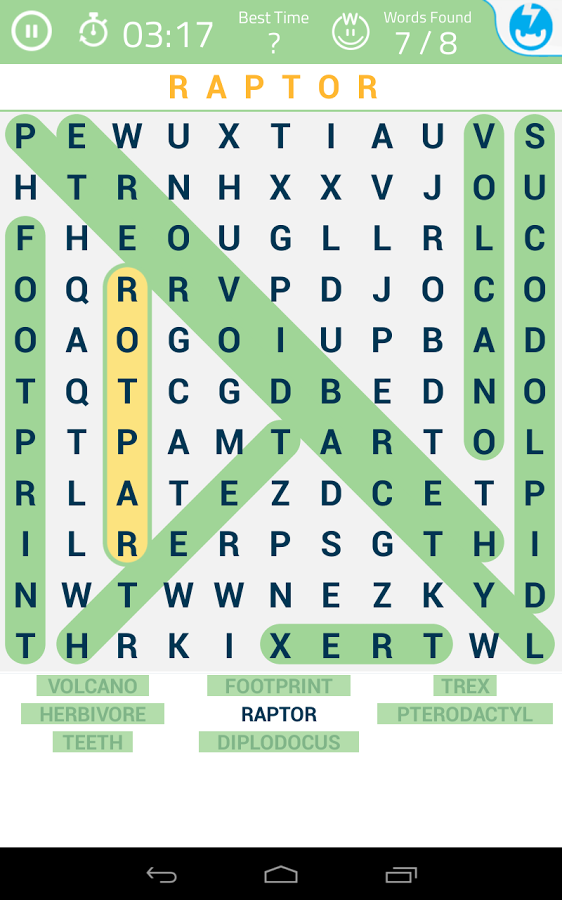
\includegraphics[scale=0.15]{word_puzzle.png}

\end{figure}
\end{column}
\end{columns}
\end{frame}

\begin{frame}\frametitle{Game Specifications}
\begin{columns}[c]
\begin{column}{5cm}
\begin{block}{User Input }
\begin{enumerate}
\item Size of grid - N
\item Difficulty level - Easy, Medium Hard
\item Dictionary - Animals, Cars
\end{enumerate}
\end{block}
\end{column}
\pause
\begin{column}{5cm}
\begin{block}{Game parameters}
\begin{enumerate}
\item Length of longest word, L
\item No. of words
\item Intersection of words, I
\item Display the set of words  
\item Random filling of characters
\end{enumerate}
\end{block}
\end{column}
\end{columns}
\pause
%\begin{table}[h!] 
\centering
%\capti\on{}
\label{tablewc}
\resizebox{\columnwidth}{!}
{

\begin{tabular}{|c|l | l | l |}
\hline
 & Easy & Medium & Hard \\
\hline
  & I- No & I- Yes & I- Yes\\
& Display - Yes & Display - Yes & Display - No  \\ \hline
\multirow{2}{*}{N = 8}  & WL - 6 &  WL- 8 & WL - 8\\
& No.of words =6 & No. of words =8 & No. of words =8\\
\hline
\multirow{2}{*}{N = 12}  & WL - 8 &  WL- 10 & WL - 10\\
& No.of words =8 & No. of words =12 & No. of words =12\\
\hline
\end{tabular}
}
\vfill
\textbf{PyGame- GUI , Python - algorithm, Wx - for options widget}
%\end{table} 
\end{frame}

\begin{frame}\frametitle {Modules}
\begin{block}{Modules}
\begin{enumerate} 
\item \textbf{Options GUI} - Gets input from user
\item \textbf{Game Settings} - Stores user input and calculates Game Design parameters 
\item \textbf{Character Matrix} - holds matrix and get and set word and random fill function
\item \textbf{Wordlist}
\begin{itemize} \item holds word list and strategically populates matrix with words  \item  chooses words and places them according to the difficulty levels \end{itemize}
\item \textbf{Game GUI} - sets up the GAME and monitors the user actions
\item \textbf{Game Status} - stores the user game state \\Eg.current - score, time, word found
\end{enumerate}
main function - which integrates all and runs the game
\end{block}
\end{frame}

\begin{frame}{Intermediate Work Done}

\begin{block}{Intermediate Work Done - Until $24^{th}$ March}
\begin{itemize}
\item Completed 3 modules with unit testing
\begin{enumerate}
\item Character Matrix
\item Word List 
\item Game GUI
\end{enumerate}
\item Difficulty level 0 - ensuring no overlaps and even spread of words
\item GUI with fixed sized window, 2 mouse clicks selects the word  
 \end{itemize}
\end{block}
\end{frame}

\begin{frame}{ScreenShots}
\begin{columns}[c]
\begin{column}{4cm}
\begin{figure}
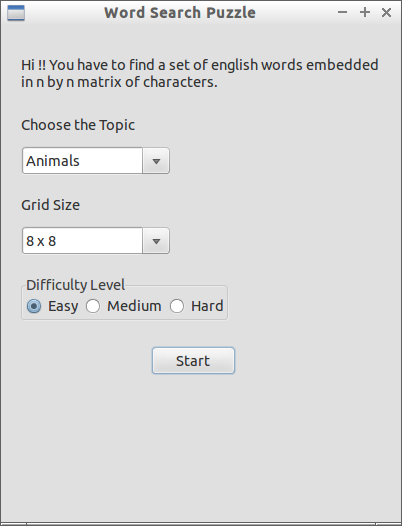
\includegraphics[scale=0.3]{opitons_gui.png}
\caption{Options Menu}
\end{figure}

\end{column}
\begin{column}{6cm}

\begin{figure}
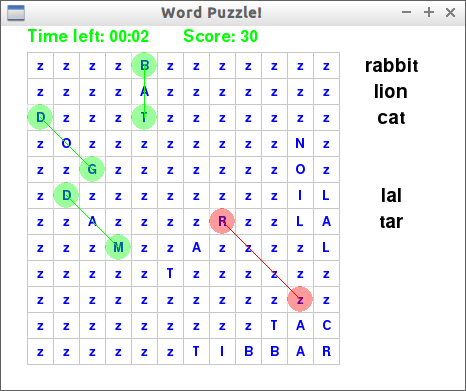
\includegraphics[scale=0.4]{puzzle_running.png}
\caption{Puzzle Running}
\end{figure}
\end{column}
\end{columns}
\end{frame}

\begin{frame}{Game Flow}
\begin{columns}[c]
\begin{column}{4cm}
\begin{tcolorbox}[colback=blue!5,colframe=blue!50!black,title=1]
\centering Start Options Menu GUI
\end{tcolorbox}
\pause
\begin{figure}
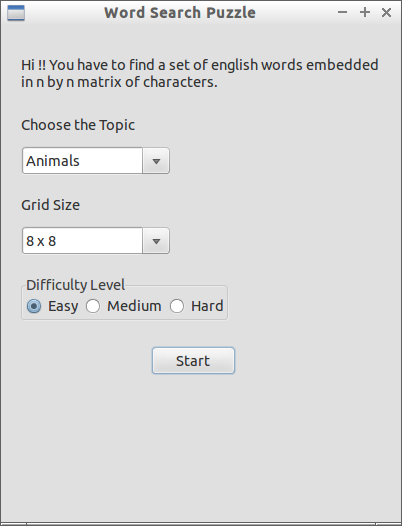
\includegraphics[scale=0.3]{opitons_gui.png}
%\caption{Options Menu}
\end{figure}
\end{column}
\pause
\begin{column}[b]{3cm}
\begin{tcolorbox}[colback=blue!5,colframe=blue!50!black, title=2]
\centering Store in \\Game Settings
\end{tcolorbox}

\end{column}
\pause
\begin{column}{3cm}
\begin{tcolorbox}[colback=blue!5,colframe=blue!50!black, title=3]
\centering Generate Word List and their Positions
\end{tcolorbox}
\pause
\begin{figure}
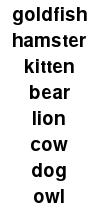
\includegraphics[scale=0.4]{word_list1.png}
%\caption{Options Menu}
\end{figure}
\end{column}

\end{columns}
\end{frame}

\begin{frame}{Game Flow - Continued}
\begin{columns}[c]

\begin{column}{3cm}
\begin{tcolorbox}[colback=blue!5,colframe=blue!50!black,title=4]
\centering Generate Character Matrix
\end{tcolorbox}
\pause
\begin{figure}
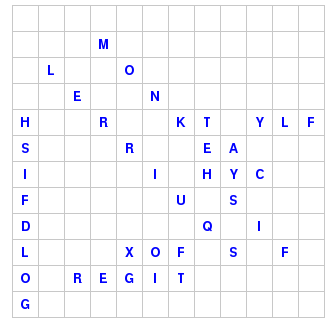
\includegraphics[scale=0.3]{char_mat2.png}
%\caption{Options Menu}
\end{figure}
\end{column}
\pause
\begin{column}[b]{4cm}
\begin{tcolorbox}[colback=blue!5,colframe=blue!50!black,title=5]
\centering Initialize Game State
\end{tcolorbox}
\pause
\begin{figure}
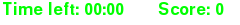
\includegraphics[scale=0.5]{game_status.png}
%\caption{}
\end{figure}
\end{column}
\pause
\begin{column}{3cm}
\begin{tcolorbox}[colback=blue!5,colframe=blue!50!black,title=6]
\centering Start Game GUI
\end{tcolorbox}
\pause
\begin{figure}
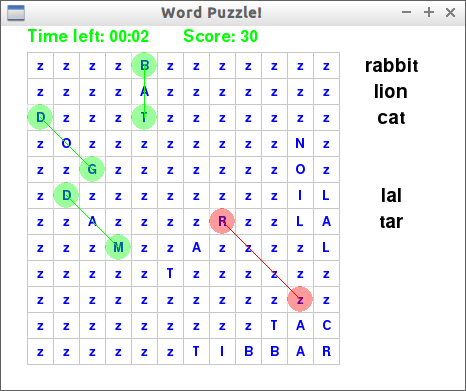
\includegraphics[scale=0.2]{puzzle_running.png}
%\caption{Options Menu}
\end{figure}
\end{column}

\end{columns}
\end{frame}

\begin{frame}{Design Strategy}
\begin{columns}[c]
\begin{column}{5cm}
\begin{block}{Design Strategy}
\begin{itemize}
\item MVC -Model View  Controller for GAME GUI
\item Divide into modules -oop design
\item Top down Approach
\end{itemize}
\end{block}
\end{column}

\begin{column}{5cm}

\begin{figure}
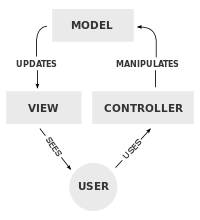
\includegraphics[scale=0.7]{mvc.png}
\caption{Model View Controller}
\end{figure}
\small{Image Source: Wikipedia}
\end{column}
\end{columns}

\end{frame}

\begin{frame}{Algo Features and Testing}
\begin{block}{Algo Features}
\begin{enumerate}
\item  Sticky Mouse Postitioning in Game GUI
\item Algorithm to find position of words to be placed. 
\end{enumerate}
\textbf{Testing}
\begin{itemize}
\item Logic and GUI has been separated as modules and developed separately
\item Separation of Concern
\item The logic has been tested using unit test.
\item Inside the modules, divided into functions and tested individually.
\end{itemize}


\end{block}


\end{frame}



\begin{frame}
\frametitle{Possible Upgrades}

\begin{itemize}
\item Enhance User experience - by improving GUI
\item Generate More diffuculty levels
\item User Memory- store the specific user settings 
\item level by level unlocking
\end{itemize}

\end{frame}


\begin{frame}{Resources}
\begin{enumerate}

\item Word Postitioning Algorithm
\begin{itemize}[]
\item \url{http://stackoverflow.com/questions/6332652/a-fast-algorithm-for-creating-a-puzzle}
\end{itemize}

\item PyGame  
\begin{itemize}[]
\item \url{inventwithpython.com/pygame/chapter2.html}

\end{itemize}

\item Wx Widget
\begin{itemize}[]
\item \url{http://wiki.wxpython.org/Getting\%20Started}
\item \url{http://zetcode.com/wxpython/}
\end{itemize}

\end{enumerate}

\end{frame}
% 

\begin{frame}
\Huge{\centerline{Thank you}}
\end{frame}





\end{document}